% ---------------------------------------------------------------------------
% Foundations of Agentic AI for Science & Engineering
% AESCAPE 2026, SC03: Introduction to Agentic Workflows
% Nathaniel Trask
%
% Build:  latexmk -pdf agentic_ai_intro.tex
%   or:   pdflatex agentic_ai_intro.tex  (twice, for the frame numbers)
% ---------------------------------------------------------------------------
\documentclass[aspectratio=169,10pt]{beamer}

\usetheme{default}
\usecolortheme{seagull}
\setbeamertemplate{navigation symbols}{}
\setbeamertemplate{itemize items}[square]
\setbeamercolor{title}{fg=black}
\setbeamercolor{frametitle}{fg=black}
\setbeamerfont{frametitle}{series=\bfseries,size=\large}
\setbeamerfont{title}{series=\bfseries}

\usepackage[T1]{fontenc}
\usepackage{lmodern}
\usepackage{amsmath,amssymb}
\usepackage{booktabs}
\usepackage{listings}
\usepackage{xcolor}
\usepackage{tikz}
\usetikzlibrary{arrows.meta,positioning,shapes.geometric,fit,backgrounds}

% --- footer -----------------------------------------------------------------
\setbeamertemplate{footline}{%
  \hfill\scriptsize\color{gray}%
  AESCAPE 2026 $\cdot$ Agentic AI $\cdot$ \insertframenumber/\inserttotalframenumber%
  \hspace*{2ex}\vspace*{1ex}%
}

% --- code style -------------------------------------------------------------
\definecolor{kw}{RGB}{0,90,160}
\definecolor{str}{RGB}{140,60,20}
\definecolor{cmt}{RGB}{110,110,110}
\definecolor{bgcode}{RGB}{247,247,247}
\definecolor{accent}{RGB}{170,30,30}

\lstdefinestyle{py}{
  language=Python,
  basicstyle=\ttfamily\scriptsize,
  keywordstyle=\color{kw}\bfseries,
  stringstyle=\color{str},
  commentstyle=\color{cmt}\itshape,
  showstringspaces=false,
  backgroundcolor=\color{bgcode},
  frame=none,
  breaklines=true,
  columns=fullflexible,
  keepspaces=true,
  aboveskip=4pt,belowskip=4pt,
  morekeywords={def,return,for,in,if,else,elif,while,try,except,class,import,from,as,with,yield,lambda,None,True,False,not,and,or}
}
\lstset{style=py}

\newcommand{\code}[1]{\texttt{\small #1}}
\newcommand{\hl}[1]{\textcolor{accent}{\textbf{#1}}}

% --- title ------------------------------------------------------------------
\title{\Large Foundations of Agentic AI\\for Science \& Engineering}
\subtitle{AESCAPE 2026 $\cdot$ SC03: Introduction to Agentic Workflows}
\author{Nathaniel Trask}
\institute{\small University of Pennsylvania}
\date{September 8, 2026}

\begin{document}

\begin{frame}[plain]
  \titlepage
\end{frame}

% ===========================================================================
\begin{frame}{Today}
\begin{enumerate}\itemsep8pt
  \item \textbf{Foundations.} What an agent is. Tools, schemas, the loop.
        Build ReAct from scratch in ${\sim}30$ lines.
  \item \textbf{The framework zoo.} ReAct, graphs (LangGraph), conversational
        multi-agent (AutoGen), MPC-style planning --- and MCP.
        \emph{Syntax, a toy, and an exemplar for each.}
  \item \textbf{Scientific computing as a tool surface.} CAD $\to$ mesh $\to$
        solve $\to$ post, re-cut so an LLM can drive it.
  \item \textbf{Reliability.} Verifier agents, manufactured solutions, oracles.
\end{enumerate}

\vfill
\begin{block}{The one question this talk is organized around}
For any given problem, \hl{which agentic pattern should you reach for, and why?}
Not ``how do I use library X.''
\end{block}
\end{frame}

% ===========================================================================
\section{Foundations}

\begin{frame}{What is an LLM agent?}
\begin{center}\large
\textbf{Agent = LLM + tools + a loop.}
\end{center}
\vspace{1em}
\begin{itemize}\itemsep6pt
  \item A bare LLM takes text in, emits text out. One shot.
  \item An \hl{agent} is an LLM running in a loop with access to \hl{tools}:
        ordinary Python functions it can ask us to run on its behalf.
  \item Each turn, the model reads the running conversation and decides to either
  \begin{itemize}
    \item emit a final text answer, or
    \item call a tool with structured arguments.
  \end{itemize}
  \item When it calls a tool, \emph{we} run the function and feed the result back
        as the next turn.
\end{itemize}
\vfill
The model never executes anything. It emits a request; you stay in control of
what actually runs.
\end{frame}

% ---------------------------------------------------------------------------
\begin{frame}{The loop, as a picture}
\begin{center}
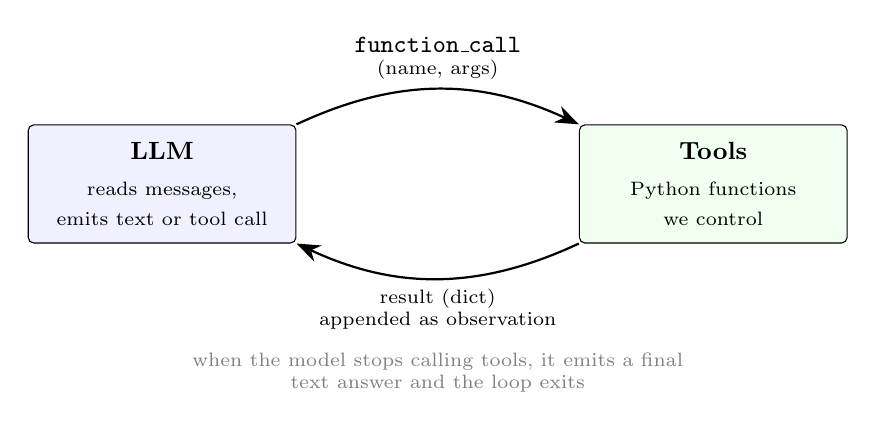
\begin{tikzpicture}[
  box/.style={draw,rounded corners=2pt,minimum width=3.4cm,minimum height=1.5cm,align=center,font=\small},
  ar/.style={-{Stealth[length=3mm]},thick}
]
\node[box,fill=blue!6] (llm) at (0,0) {\textbf{LLM}\\[2pt]\scriptsize reads messages,\\\scriptsize emits text or tool call};
\node[box,fill=green!6] (tool) at (7,0) {\textbf{Tools}\\[2pt]\scriptsize Python functions\\\scriptsize we control};

\draw[ar] (llm.north east) to[bend left=25]
  node[above,font=\scriptsize,align=center]{\code{function\_call}\\(name, args)} (tool.north west);
\draw[ar] (tool.south west) to[bend left=25]
  node[below,font=\scriptsize,align=center]{result (dict)\\appended as observation} (llm.south east);

\node[font=\scriptsize,align=center,gray] at (3.5,-2.4)
  {when the model stops calling tools, it emits a final\\text answer and the loop exits};
\end{tikzpicture}
\end{center}
\vspace{-0.3em}
\begin{center}
This is \hl{ReAct} (Reason + Act), Yao et al.\ 2022 --- the simplest agent there is.
\end{center}
\end{frame}

% ---------------------------------------------------------------------------
\begin{frame}[fragile]{What a tool is}
Two pieces, both written by you: a Python function, and a JSON-schema
description of its signature that you hand to the model.

\vspace{0.5em}
\begin{columns}[T,onlytextwidth]
\begin{column}{0.47\textwidth}
{\footnotesize\textbf{Python function} (you call it)}
\begin{lstlisting}
def calculator(op, a, b):
    ops = {"add": a + b, "sub": a - b,
           "mul": a * b, "div": a / b}
    return {"result": ops[op]}
\end{lstlisting}
\end{column}
\begin{column}{0.5\textwidth}
{\footnotesize\textbf{JSON schema} (the model reads it)}
\begin{lstlisting}
{"name": "calculator",
 "description": "One arithmetic op.",
 "parameters": {
   "type": "object",
   "properties": {
     "op": {"type": "string",
            "enum": ["add","sub","mul","div"]},
     "a": {"type": "number"},
     "b": {"type": "number"}},
   "required": ["op","a","b"]}}
\end{lstlisting}
\end{column}
\end{columns}

\vspace{0.5em}
\begin{itemize}\itemsep2pt\small
  \item \code{name}, \code{description} --- decide whether the model picks
        \emph{this} tool over the others. This is prompt engineering; write it carefully.
  \item \code{properties} --- the typed argument list. \code{enum} restricts a
        string to a fixed set. Constrain aggressively: every value you forbid in the
        schema is a failure mode you never have to debug.
\end{itemize}
\end{frame}

% ---------------------------------------------------------------------------
\begin{frame}[fragile]{The round trip}
Each turn, the model emits either plain text (final answer) or a structured tool call.

\vspace{0.5em}
\textbf{1.} The reply contains a \code{function\_call} part:
\begin{lstlisting}
response.candidates[0].content.parts[0].function_call
    .name = "calculator"
    .args = {"op": "mul", "a": 13, "b": 47}
\end{lstlisting}

\textbf{2.} We dispatch by name and run the Python function:
\begin{lstlisting}
result = tool_fns[name](**args)          # -> {"result": 611}
\end{lstlisting}

\textbf{3.} We send the result back as a \code{function\_response} on the next turn:
\begin{lstlisting}
Part.from_function_response(name="calculator", response={"result": 611})
\end{lstlisting}

\vspace{0.3em}
The model then sees its own call, the result, and decides whether to call
another tool or stop.
\end{frame}

% ---------------------------------------------------------------------------
\begin{frame}[fragile]{The whole thing, in pseudocode}
\begin{lstlisting}
def run_agent(system_prompt, user_prompt, tool_schemas, tool_fns, max_steps=12):
    messages = [user_prompt]
    for step in range(max_steps):
        response = llm(system_prompt, messages, tools=tool_schemas)
        messages.append(response)

        if response.is_tool_call:
            for call in response.tool_calls:
                try:
                    result = tool_fns[call.name](**call.args)
                except Exception as e:
                    result = {"error": str(e)}      # errors are observations
                messages.append(result)
        else:
            return response.text                    # final answer
\end{lstlisting}

\vspace{0.5em}
That is a complete agent. Everything else in this talk is a variation on
\hl{who decides what happens next}.
\end{frame}

% ---------------------------------------------------------------------------
\begin{frame}[fragile]{Two slots: \code{system\_prompt} vs \code{user\_prompt}}
\begin{itemize}\itemsep6pt
  \item \hl{\code{system\_prompt}} --- the \emph{rules of the game}. Identity,
        methodology, what the tools are for, budgets, how to stop. Sent on every
        turn as a persistent header; never drowned out as observations pile up.
  \item \hl{\code{user\_prompt}} --- the \emph{specific ask} that triggers this
        run. Becomes the first message; tool calls and observations append after it.
\end{itemize}

\vspace{0.5em}
\begin{lstlisting}
B1_SYSTEM = """You optimize a black-box function (angle in degrees, in (0,90))
returning a range in meters. Budget: at most 12 evaluate() calls. Use history if
helpful, then call propose_answer with your guess."""

B1_USER = "Find the optimal angle. Budget: 12 evaluations."
\end{lstlisting}

\vspace{0.5em}
Rule of thumb: durable rules about \emph{how to behave} go in the system prompt;
the specific \emph{thing to do this run} goes in the user prompt.
\end{frame}

% ---------------------------------------------------------------------------
\begin{frame}[fragile]{Errors are observations, not crashes}
Tool calls \emph{will} fail. The model invents an argument, asks for a mesh ID
that does not exist, passes a string where you wanted a float.

\begin{lstlisting}
try:
    result = tool_fns[name](**args)
except Exception as e:
    result = {"error": f"{type(e).__name__}: {e}"}
\end{lstlisting}

\vspace{0.5em}
The model reads the error on the next turn and, with a reasonable prompt,
retries with correct arguments.

\vfill
\begin{block}{You will see this happen live today}
An agent recovering from its own bad tool call is the system working, not the
system failing. The failure mode to actually fear is on slide
``agents are confidently wrong.''
\end{block}
\end{frame}

% ---------------------------------------------------------------------------
\begin{frame}{Guardrails belong in the tool, not the prompt}
A prompt is a request. A tool is an enforcement point.

\vspace{0.8em}
\begin{center}
\begin{tabular}{ll}
\toprule
\textbf{Hope} (prompt) & \textbf{Guarantee} (tool) \\
\midrule
``don't refine past 20k DOFs'' & \code{if new\_dofs > MAX\_DOFS: return \{"error": ...\}} \\
``use at most 12 evaluations'' & counter in the tool; refuse call 13 \\
``don't touch the boundary'' & tool has no boundary argument \\
``stop when converged''       & \code{stop()} is the only terminal tool \\
\bottomrule
\end{tabular}
\end{center}

\vspace{1em}
Anything you would be unwilling to let a nondeterministic process do,
\hl{make impossible in the tool signature} --- do not ask nicely in English.

\vspace{0.5em}
This is the single highest-leverage habit for making agentic workflows safe
enough to run unattended.
\end{frame}

% ---------------------------------------------------------------------------
\begin{frame}{Setup: getting a key}
\begin{enumerate}\itemsep6pt
  \item \textbf{Free, no credit card.} Google AI Studio:
        \url{https://aistudio.google.com/apikey}. Sign in with any Google account.
        Use a project where billing has \emph{never} been enabled.
  \item \textbf{Bring your own.} Anthropic
        (\url{https://console.anthropic.com}) or OpenAI
        (\url{https://platform.openai.com/api-keys}) both work.
  \item In Colab: \textbf{Secrets} panel (key icon, left sidebar), add
        \code{GEMINI\_API\_KEY}. Locally: \code{export GEMINI\_API\_KEY=...}
  \item Run the Part 0 cells to confirm the client connects.
\end{enumerate}

\vfill
\begin{block}{Never paste a key into a notebook cell}
It ends up in the \code{.ipynb} JSON, in your shell history, and in git.
Use the secrets panel or an environment variable.
\end{block}
\end{frame}

% ===========================================================================
\section{The framework zoo}

\begin{frame}[plain]
\begin{center}
\Huge\bfseries The framework zoo
\vspace{1em}

\large\mdseries ReAct $\cdot$ LangGraph $\cdot$ AutoGen $\cdot$ MPC $\cdot$ MCP
\end{center}
\end{frame}

% ---------------------------------------------------------------------------
\begin{frame}{Why not just ReAct?}
ReAct is greedy. At each step the model sees the history and picks one action.
That is exactly right when:

\begin{itemize}\itemsep4pt
  \item the tool surface is small,
  \item mistakes are cheap and recoverable, and
  \item you cannot specify the procedure in advance.
\end{itemize}

\vspace{0.8em}
It starts to hurt when:

\begin{itemize}\itemsep4pt
  \item you need a \hl{guarantee} that step B always follows step A
        (audit, compliance, ``always verify before reporting''),
  \item genuinely \hl{different expertise} needs different system prompts and
        different tools,
  \item a wrong action is \hl{expensive} and you own a cheap forward model that
        could have caught it, or
  \item your tools live in \hl{someone else's process} --- a solver, a CAD kernel,
        a database.
\end{itemize}

\vspace{0.5em}
Each of those pressures produced a different pattern. That is the zoo.
\end{frame}

% ---------------------------------------------------------------------------
\begin{frame}{The only question that matters}
\begin{center}
{\Large Choosing a pattern is choosing \hl{who owns control flow}.}
\end{center}

\vspace{1.2em}
\begin{center}
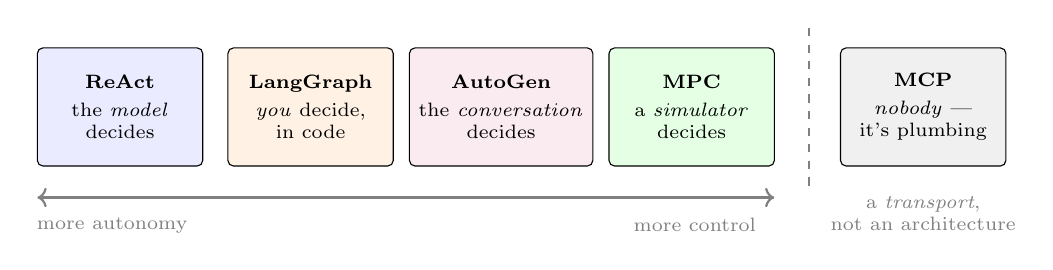
\begin{tikzpicture}[
  n/.style={draw,rounded corners=2pt,minimum width=2.1cm,minimum height=1.5cm,align=center,font=\scriptsize},
  every node/.style={align=center}
]
\node[n,fill=blue!8]   (a) at (0,0)    {\textbf{ReAct}\\[2pt]the \emph{model}\\decides};
\node[n,fill=orange!10](b) at (2.42,0) {\textbf{LangGraph}\\[2pt]\emph{you} decide,\\in code};
\node[n,fill=purple!8] (c) at (4.84,0) {\textbf{AutoGen}\\[2pt]the \emph{conversation}\\decides};
\node[n,fill=green!10] (d) at (7.26,0) {\textbf{MPC}\\[2pt]a \emph{simulator}\\decides};

\draw[dashed,gray] (8.75,-1.0) -- (8.75,1.0);
\node[n,fill=gray!12]  (e) at (10.2,0) {\textbf{MCP}\\[2pt]\emph{nobody} ---\\it's plumbing};

\draw[<->,thick,gray] (-1.05,-1.15) -- (8.31,-1.15);
\node[font=\scriptsize,gray] at (-0.1,-1.5) {more autonomy};
\node[font=\scriptsize,gray] at (7.3,-1.5) {more control};
\node[font=\scriptsize,gray,align=center] at (10.2,-1.35) {a \emph{transport},\\not an architecture};
\end{tikzpicture}
\end{center}

\vspace{0.8em}
MCP sits apart on purpose: it is a \emph{transport}, not an architecture.
You can use it with any of the other four. (More on the unfortunate
MPC/MCP name collision shortly.)
\end{frame}

% ---------------------------------------------------------------------------
\begin{frame}{The zoo, on one slide}
\begin{center}\small
\begin{tabular}{@{}lllll@{}}
\toprule
 & \textbf{Control flow} & \textbf{Lookahead} & \textbf{Roles} & \textbf{Reach for it when} \\
\midrule
\textbf{ReAct}
  & model, step by step & none & one
  & open-ended, errors cheap \\[3pt]
\textbf{LangGraph}
  & you, as a graph & none & many, fixed
  & you need guarantees \\[3pt]
\textbf{AutoGen}
  & emergent, via chat & none & many, fluid
  & expertise must collide \\[3pt]
\textbf{MPC}
  & simulator ranks plans & $N$ steps & one + model
  & wrong actions are costly \\[3pt]
\midrule
\textbf{MCP}
  & \multicolumn{4}{l}{\emph{orthogonal} --- how tools reach the agent, not how it decides} \\
\bottomrule
\end{tabular}
\end{center}

\vspace{1em}
For each of the four architectures we will look at:
\begin{enumerate}\itemsep2pt
  \item the \textbf{syntax} --- what the code actually looks like,
  \item a \textbf{toy} --- the same trivial task, so the comparison is fair,
  \item an \textbf{exemplar} --- a problem where that pattern genuinely wins.
\end{enumerate}
\end{frame}

% ---------------------------------------------------------------------------
\begin{frame}{The common toy task}
To compare syntax fairly, every framework gets the \emph{same} trivial job:

\vspace{0.8em}
\begin{center}
\begin{minipage}{0.75\textwidth}
\begin{block}{Toy task}
Given a target number, use a \code{calculator} tool to reach it, then report
the result. No framework should need more than ${\sim}20$ lines.
\end{block}
\end{minipage}
\end{center}

\vspace{1em}
The toy is deliberately too easy to justify any of them. That is the point:
when the task is trivial, all four look like unnecessary ceremony, and you
can see the raw syntax without the problem getting in the way.

\vspace{0.8em}
Then each \textbf{exemplar} shows the task where the ceremony pays for itself.

\vfill
\begin{center}\small\color{gray}
Notebook: \code{01\_agentic\_patterns.ipynb}, \S1--\S5
\end{center}
\end{frame}

% ===========================================================================
% ---- PATTERN 1: ReAct -----------------------------------------------------
\begin{frame}[plain]
\begin{center}
{\Large\bfseries Pattern 1 --- ReAct}\\[0.5em]
{\large\color{gray} the model owns control flow}
\end{center}
\end{frame}

\begin{frame}[fragile]{ReAct --- syntax}
No framework. A \code{for} loop and a dispatch table.

\begin{lstlisting}
contents = [user_prompt]
for step in range(max_steps):
    resp = client.models.generate_content(
        model=MODEL, contents=contents,
        config=GenerateContentConfig(
            system_instruction=system_prompt,
            tools=[Tool(function_declarations=tool_schemas)]))
    contents.append(resp.candidates[0].content)

    calls = [p.function_call for p in resp.candidates[0].content.parts
             if p.function_call]
    if not calls:
        return resp.text                       # final answer

    for fc in calls:
        result = tool_fns[fc.name](**dict(fc.args))
        contents.append(Part.from_function_response(
            name=fc.name, response=result))
\end{lstlisting}
\vspace{-0.3em}
{\small Dependencies: one SDK. State: the \code{contents} list. That's it.}
\end{frame}

\begin{frame}{ReAct --- exemplar: adaptive mesh refinement}
\begin{columns}[T,onlytextwidth]
\begin{column}{0.55\textwidth}
\textbf{Why ReAct is the right call here:}
\begin{itemize}\itemsep5pt\small
  \item The number of refinement cycles is \hl{not knowable in advance} ---
        it depends on observed error.
  \item Every action is \hl{cheap and recoverable}: a bad refinement just makes
        a mesh you discard.
  \item The model must \hl{react to observations} it could not have predicted
        (the error estimate after each solve).
  \item The tool surface is \hl{small} --- six tools.
\end{itemize}
\vspace{0.5em}
Greedy, one-step-at-a-time decision making is not a compromise here.
It is the correct algorithm.
\end{column}
\begin{column}{0.42\textwidth}
\begin{center}
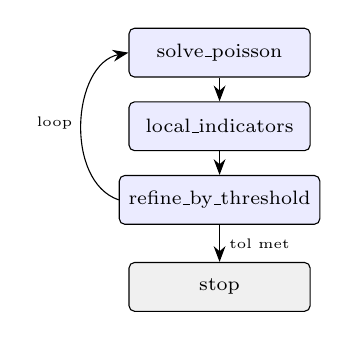
\begin{tikzpicture}[scale=0.85,
  n/.style={draw,rounded corners=2pt,minimum width=2.3cm,minimum height=0.62cm,font=\scriptsize,align=center},
  ar/.style={-{Stealth[length=2mm]}}]
\node[n,fill=blue!8]  (s) at (0,0)    {solve\_poisson};
\node[n,fill=blue!8]  (i) at (0,-1.1) {local\_indicators};
\node[n,fill=blue!8]  (r) at (0,-2.2) {refine\_by\_threshold};
\node[n,fill=gray!12] (t) at (0,-3.5) {stop};
\draw[ar] (s) -- (i);
\draw[ar] (i) -- (r);
\draw[ar] (r.west) to[bend left=75] node[left,font=\tiny]{loop} (s.west);
\draw[ar] (r) -- node[right,font=\tiny]{tol met} (t);
\end{tikzpicture}
\end{center}
\vspace{0.3em}
{\scriptsize\color{gray} The model chooses the arrow to take at every step.
Nothing in the code forces this order.}
\end{column}
\end{columns}
\end{frame}

% ---- PATTERN 2: LangGraph -------------------------------------------------
\begin{frame}[plain]
\begin{center}
{\Large\bfseries Pattern 2 --- Graphs (LangGraph)}\\[0.5em]
{\large\color{gray} you own control flow}
\end{center}
\end{frame}

\begin{frame}[fragile]{LangGraph --- syntax}
You declare a typed state, nodes that transform it, and edges. The LLM fills
in nodes; \emph{the graph} decides what runs next.

\begin{lstlisting}
from langgraph.graph import StateGraph, END
from typing import TypedDict

class S(TypedDict):
    mesh_id: int
    error: float
    attempts: int

def solve(s):  return {"error": run_solver(s["mesh_id"]), ...}
def refine(s): return {"mesh_id": do_refine(s["mesh_id"]),
                       "attempts": s["attempts"] + 1}

def route(s):                                  # <- control flow, in Python
    if s["error"] < TOL:      return "verify"
    if s["attempts"] >= 6:    return "give_up"
    return "refine"

g = StateGraph(S)
g.add_node("solve", solve); g.add_node("refine", refine)
g.add_node("verify", verify)
g.set_entry_point("solve")
g.add_conditional_edges("solve", route,
    {"refine": "refine", "verify": "verify", "give_up": END})
g.add_edge("refine", "solve")
app = g.compile()
\end{lstlisting}
\end{frame}

\begin{frame}{LangGraph --- what you actually bought}
\begin{columns}[T,onlytextwidth]
\begin{column}{0.52\textwidth}
\textbf{Guarantees, not suggestions:}
\begin{itemize}\itemsep5pt\small
  \item \code{verify} \hl{always} runs before a result is reported.
        The model cannot decide to skip it.
  \item The retry count is \hl{bounded in code}. No prompt can talk it into a
        seventh attempt.
  \item State is \hl{typed and inspectable} --- you can log, checkpoint, and
        resume mid-run.
  \item The control flow is a \hl{diagram you can show a reviewer}, which
        matters when the answer feeds a design decision.
\end{itemize}
\end{column}
\begin{column}{0.45\textwidth}
\begin{center}
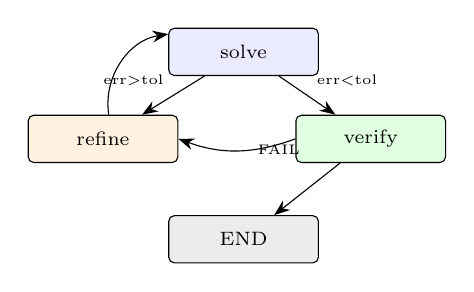
\begin{tikzpicture}[scale=0.85,
  n/.style={draw,rounded corners=2pt,minimum width=1.9cm,minimum height=0.6cm,font=\scriptsize,align=center},
  ar/.style={-{Stealth[length=2mm]}}]
\node[n,fill=blue!8]   (s) at (0,0)      {solve};
\node[n,fill=orange!12](r) at (-2.1,-1.3){refine};
\node[n,fill=green!12] (v) at (1.9,-1.3) {verify};
\node[n,fill=gray!15]  (e) at (0,-2.8)   {END};
\draw[ar] (s) -- node[above left,font=\tiny]{err>tol} (r);
\draw[ar] (s) -- node[above right,font=\tiny]{err<tol} (v);
\draw[ar] (r) to[bend left=45] (s);
\draw[ar] (v) -- (e);
\draw[ar] (v.west) to[bend left=20] node[right,font=\tiny,pos=0.4]{FAIL} (r.east);
\end{tikzpicture}
\end{center}
\vspace{0.5em}
{\scriptsize\color{gray} Compare with the ReAct diagram: same boxes, but here
the \emph{arrows are code}. The model never sees them.}
\end{column}
\end{columns}
\end{frame}

\begin{frame}{LangGraph --- exemplar: solve $\to$ verify $\to$ repair}
\textbf{The problem:} you want an FEM result you can put in a report.

\vspace{0.8em}
\begin{center}\small
\begin{tabular}{@{}ll@{}}
\toprule
\textbf{Requirement} & \textbf{Who enforces it} \\
\midrule
Every reported result is verified & the graph, not the prompt \\
At most 6 refinement attempts & the router, in Python \\
A failed verification triggers repair, not a retry & a conditional edge \\
The whole run is reproducible from a checkpoint & typed state \\
\bottomrule
\end{tabular}
\end{center}

\vspace{1em}
None of these are things you want a language model deciding on a given Tuesday.
When ``it usually does the right thing'' is not good enough, you stop asking and
start wiring.

\vspace{0.8em}
\begin{center}
\hl{Reach for a graph when the control flow is a requirement, not a choice.}
\end{center}
\end{frame}

% ---- PATTERN 3: AutoGen ---------------------------------------------------
\begin{frame}[plain]
\begin{center}
{\Large\bfseries Pattern 3 --- Conversational multi-agent (AutoGen)}\\[0.5em]
{\large\color{gray} the conversation owns control flow}
\end{center}
\end{frame}

\begin{frame}[fragile]{AutoGen --- syntax}
You define participants with distinct system prompts and let them talk. Control
flow emerges from who speaks next.

\begin{lstlisting}
from autogen_agentchat.agents import AssistantAgent
from autogen_agentchat.teams import RoundRobinGroupChat
from autogen_agentchat.conditions import TextMentionTermination

modeler = AssistantAgent("modeler", model_client=client,
    system_message="You propose discretizations. Be concrete and specific.")

analyst = AssistantAgent("analyst", model_client=client,
    system_message="""You are a numerical analyst. Challenge the modeler's
    proposal on stability, conditioning, and convergence rate. Do not be
    agreeable; your value is in the objection.""")

critic = AssistantAgent("critic", model_client=client,
    system_message="Judge the exchange. Say APPROVE only when convinced.")

team = RoundRobinGroupChat([modeler, analyst, critic],
    termination_condition=TextMentionTermination("APPROVE"))

await team.run(task="Choose a discretization for advection-dominated flow.")
\end{lstlisting}
\end{frame}

\begin{frame}{AutoGen --- exemplar: the design review}
\textbf{The problem:} choosing a discretization for an advection-dominated
problem. There is no single correct answer, and the \emph{reasoning} is the
deliverable.

\vspace{0.8em}
\begin{itemize}\itemsep5pt
  \item A single ReAct agent asked ``pick a discretization'' produces a
        confident paragraph with no adversarial pressure on it.
  \item Three agents with \hl{genuinely different objectives} --- propose,
        object, judge --- produce a transcript in which the weaknesses are
        stated out loud.
  \item The artifact is not the answer. It is \hl{the argument}, which a human
        can audit far faster than they can re-derive.
\end{itemize}

\vspace{1em}
\begin{center}
\hl{Reach for conversation when disagreement is the product.}
\end{center}

\vspace{0.5em}
{\small\color{gray}Caveat worth stating plainly: this pattern is the easiest of
the four to fool yourself with. Three LLMs agreeing is not three experts
agreeing --- they share a prior. Distinct \emph{tools} per role helps far more
than distinct adjectives in the system prompt.}
\end{frame}

% ---- PATTERN 4: MPC -------------------------------------------------------
\begin{frame}[plain]
\begin{center}
{\Large\bfseries Pattern 4 --- MPC-style planning}\\[0.5em]
{\large\color{gray} a simulator owns control flow}
\end{center}
\end{frame}

\begin{frame}{MPC --- the idea, borrowed from control}
Model Predictive Control, as you already know it:

\begin{center}
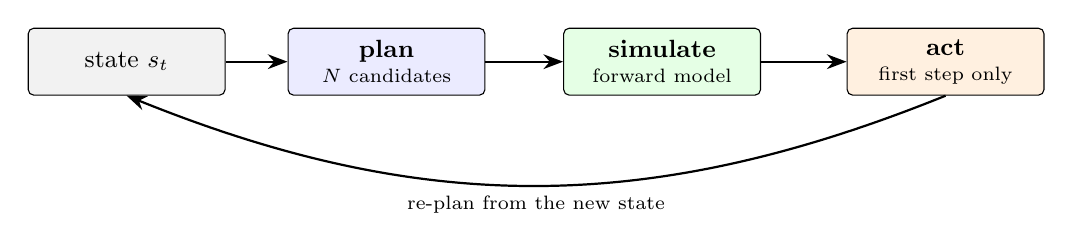
\begin{tikzpicture}[
  n/.style={draw,rounded corners=2pt,minimum width=2.5cm,minimum height=0.85cm,font=\small,align=center},
  ar/.style={-{Stealth[length=2.5mm]},thick}]
\node[n,fill=gray!10]   (s) at (0,0)    {state $s_t$};
\node[n,fill=blue!8]    (p) at (3.3,0)  {\textbf{plan}\\[-2pt]\scriptsize $N$ candidates};
\node[n,fill=green!10]  (m) at (6.8,0)  {\textbf{simulate}\\[-2pt]\scriptsize forward model};
\node[n,fill=orange!12] (a) at (10.4,0) {\textbf{act}\\[-2pt]\scriptsize first step only};
\draw[ar] (s) -- (p);
\draw[ar] (p) -- (m);
\draw[ar] (m) -- (a);
\draw[ar] (a.south) to[bend left=22] node[below,font=\scriptsize]{re-plan from the new state} (s.south);
\end{tikzpicture}
\end{center}

\vspace{0.8em}
The agentic version swaps one box: \hl{the LLM proposes the candidate plans},
and the simulator --- not the LLM --- ranks them.

\vspace{0.8em}
\begin{itemize}\itemsep3pt
  \item The LLM contributes what it is good at: \emph{proposing plausible
        candidates} from context.
  \item The simulator contributes what it is good at: \emph{being right}.
  \item You commit only to the first action, then re-plan with real feedback.
\end{itemize}
\end{frame}

\begin{frame}[fragile]{MPC --- syntax}
No library needed. The pattern is the loop.

\begin{lstlisting}
state = initial_state
for t in range(horizon):
    # 1. LLM proposes N candidate action sequences (cheap, creative)
    plans = llm_propose(state, history, n_candidates=5, lookahead=3)

    # 2. The *simulator* scores each one (trusted, not creative)
    scores = [world_model.rollout(state, plan) for plan in plans]

    # 3. Commit to the first action of the best plan only
    best = plans[argmax(scores)]
    state = env.step(best[0])            # <- the only real action taken

    # 4. Re-plan from the new state (closes the loop on reality)
\end{lstlisting}

\vspace{0.5em}
Note what the LLM never does: \hl{it never decides which plan is best}.
It generates hypotheses; the forward model adjudicates. That division is the
entire value of the pattern.
\end{frame}

\begin{frame}{MPC --- exemplar: black-box optimization}
\textbf{The problem:} find the launch angle maximizing range for a projectile
under quadratic drag. The agent sees only \code{evaluate(angle)}.

\vspace{0.6em}
$$\ddot{x} = -c_d|v|\dot{x}, \qquad \ddot{y} = -g - c_d|v|\dot{y},
\qquad v_0 = 50\,\text{m/s},\; c_d = 0.01\,\text{m}^{-1}$$

\vspace{0.6em}
\begin{itemize}\itemsep4pt
  \item Without drag the optimum is $45^\circ$; with drag it shifts lower.
        The model's prior is \emph{almost} right, which is the interesting case.
  \item Every \code{evaluate} call is a real ODE integration --- the thing we
        are budgeting.
  \item We have a \hl{cheap, trusted forward model}: the simulator itself.
\end{itemize}

\vspace{0.8em}
\begin{center}
In the notebook we run \hl{ReAct vs.\ MPC head to head on the same budget}
and count evaluations to a fixed tolerance.
\end{center}

\vspace{0.4em}
{\small\color{gray}This is the honest way to answer ``when would I reach for
one over the other'' --- measure it, don't assert it.}
\end{frame}

\begin{frame}{MPC --- when it wins, and when it doesn't}
\begin{columns}[T,onlytextwidth]
\begin{column}{0.48\textwidth}
\textbf{Reach for MPC when:}
\begin{itemize}\itemsep4pt\small
  \item A wrong action is \hl{expensive or irreversible} --- burning budget,
        committing a mesh, running an experiment.
  \item You have a \hl{cheap forward model you trust} more than the LLM.
  \item Actions compose, so looking $N$ steps ahead genuinely differs from
        looking one step ahead.
\end{itemize}
\end{column}
\begin{column}{0.48\textwidth}
\textbf{Don't bother when:}
\begin{itemize}\itemsep4pt\small
  \item Simulating a plan costs about what executing it costs --- then just
        execute and observe.
  \item You have no forward model. Then MPC degenerates into the LLM grading
        its own homework, which is worse than ReAct because it is
        \emph{slower} and equally wrong.
  \item The problem is convex and small. Use \code{scipy.optimize} and go home.
\end{itemize}
\end{column}
\end{columns}

\vfill
\begin{block}{The uncomfortable baseline}
For the projectile, \code{minimize\_scalar} finds the optimum in ${\sim}12$
evaluations with no LLM at all. We run it in the notebook. If an agent cannot
beat \code{scipy}, that is worth knowing --- and worth saying out loud.
\end{block}
\end{frame}

% ---- PATTERN 5: MCP -------------------------------------------------------
\begin{frame}[plain]
\begin{center}
{\Large\bfseries Pattern 5 --- MCP}\\[0.5em]
{\large\color{gray} not an architecture at all}
\end{center}
\end{frame}

\begin{frame}{MPC is not MCP}
\begin{center}\large
Two three-letter acronyms, one letter apart, both in this talk. Sorry.
\end{center}

\vspace{1em}
\begin{center}
\begin{tabular}{@{}p{0.44\textwidth}p{0.48\textwidth}@{}}
\toprule
\textbf{MPC} --- Model Predictive Control & \textbf{MCP} --- Model Context Protocol \\
\midrule
A \emph{control strategy}. & A \emph{wire protocol}. \\[4pt]
Borrowed from process control, 1970s. & Introduced by Anthropic, 2024. \\[4pt]
Answers: \emph{how do I decide what to do next?} & Answers: \emph{how does my agent reach a tool that lives somewhere else?} \\[4pt]
Changes your agent's reasoning. & Changes your agent's plumbing. \\
\bottomrule
\end{tabular}
\end{center}

\vspace{1em}
\begin{center}
They are orthogonal. You can --- and often should --- run an
\hl{MPC-style agent whose tools are served over MCP}.
\end{center}
\end{frame}

\begin{frame}{MCP --- the problem it solves}
So far, every tool has been a Python function in the same process as the loop.
That does not survive contact with a real simulation stack.

\vspace{0.8em}
\textbf{Your solver is:} a compiled binary. On a cluster. Behind a scheduler.
Written by someone else, in Fortran, in 1994. Licensed per seat.

\vspace{0.8em}
\begin{center}
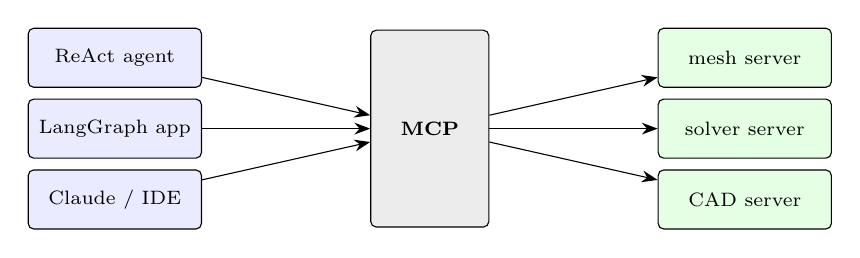
\begin{tikzpicture}[
  n/.style={draw,rounded corners=2pt,minimum width=2.2cm,minimum height=0.75cm,font=\scriptsize,align=center},
  ar/.style={-{Stealth[length=2mm]}}]
\node[n,fill=blue!8]  (c1) at (0,0.9)  {ReAct agent};
\node[n,fill=blue!8]  (c2) at (0,0)    {LangGraph app};
\node[n,fill=blue!8]  (c3) at (0,-0.9) {Claude / IDE};
\node[n,fill=gray!15,minimum height=2.5cm,minimum width=1.5cm] (p) at (4,0) {\textbf{MCP}};
\node[n,fill=green!10](s1) at (8,0.9)  {mesh server};
\node[n,fill=green!10](s2) at (8,0)    {solver server};
\node[n,fill=green!10](s3) at (8,-0.9) {CAD server};
\foreach \c in {c1,c2,c3} \draw[ar] (\c) -- (p);
\foreach \s in {s1,s2,s3} \draw[ar] (p) -- (\s);
\end{tikzpicture}
\end{center}

\vspace{0.5em}
MCP standardizes the contract between the two sides: \hl{write your solver's
tool surface once}, and any MCP-speaking client can drive it --- your notebook
today, a colleague's LangGraph pipeline tomorrow, a desktop assistant after that.
\end{frame}

\begin{frame}[fragile]{MCP --- syntax}
Server side: decorate the functions you want to expose.

\begin{lstlisting}
from mcp.server.fastmcp import FastMCP

mcp = FastMCP("fem-tools")

@mcp.tool()
def solve_poisson(mesh_id: int) -> dict:
    """Solve -Laplacian(u) = 1 with u=0 on the boundary."""
    u, basis = solve_poisson_on(MESH_REGISTRY[mesh_id])
    return {"dofs": int(basis.N), "H1_error": h1_error(...)}

@mcp.tool()
def refine_by_threshold(mesh_id: int, theta: float = 0.5) -> dict:
    """Doerfler-mark and refine. theta in (0,1)."""
    ...

mcp.run()          # now speaks MCP over stdio or HTTP
\end{lstlisting}

\vspace{0.5em}
The type hints and docstrings \emph{become} the JSON schema. Notice this is the
same information as slide ``what a tool is'' --- MCP does not change what a tool
is, only \hl{who can reach it}.
\end{frame}

\begin{frame}{Choosing: a decision guide}
\begin{center}\small
\begin{tabular}{@{}p{0.53\textwidth}p{0.42\textwidth}@{}}
\toprule
\textbf{If this is true of your problem\ldots} & \textbf{start here} \\
\midrule
I can't specify the procedure in advance, and mistakes are cheap
  & \textbf{ReAct} \\[4pt]
Something must \emph{always} happen (verify, log, approve), or a human signs off on the result
  & \textbf{LangGraph} \\[4pt]
The roles need different tools and different incentives, and I want the disagreement on record
  & \textbf{AutoGen} \\[4pt]
Actions are expensive or irreversible, and I own a forward model
  & \textbf{MPC} \\[4pt]
My tools live in another process, language, or machine --- or others need to reuse them
  & \textbf{MCP} (with any of the above) \\
\bottomrule
\end{tabular}
\end{center}

\vspace{1em}
\begin{center}
\hl{Start at the top.} Every row down is more machinery, more failure surface,
and more code you own. Earn each step.
\end{center}
\end{frame}

\begin{frame}{A word on framework enthusiasm}
All four patterns are ${\sim}30$ lines of Python. The frameworks add
persistence, retries, streaming, tracing, and a community --- real value, at
the cost of an abstraction between you and the loop.

\vspace{1em}
\begin{center}
\begin{minipage}{0.85\textwidth}
\begin{block}{Suggested order of operations}
\begin{enumerate}\itemsep2pt
  \item Write the loop yourself, once, for your problem. It is an afternoon.
  \item Find out which part actually hurts (state? retries? observability?).
  \item \emph{Then} adopt the framework that fixes that specific pain.
\end{enumerate}
\end{block}
\end{minipage}
\end{center}

\vspace{1em}
In today's notebook every pattern appears \hl{twice}: once in the real
framework's syntax, and once in ${\sim}15$ lines of plain Python. The second
version is there to demystify the first --- and so the notebook still runs when
a \code{pip install} fails on conference wifi.
\end{frame}

% ===========================================================================
\section{Scientific computing as a tool surface}

\begin{frame}[plain]
\begin{center}
\Huge\bfseries Scientific computing\\as a tool surface
\end{center}
\end{frame}

\begin{frame}{The workflow you already know}
\begin{center}
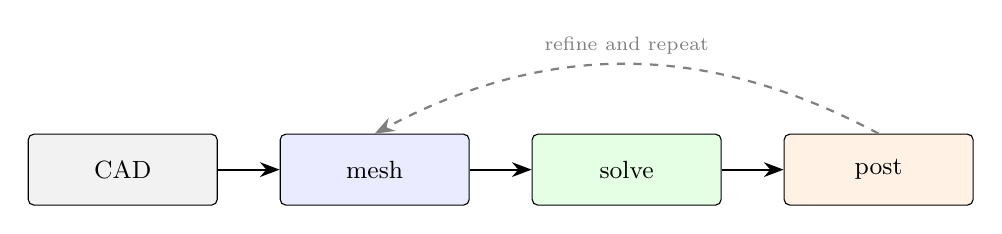
\begin{tikzpicture}[
  n/.style={draw,rounded corners=2pt,minimum width=2.4cm,minimum height=0.9cm,font=\small,align=center},
  ar/.style={-{Stealth[length=2.5mm]},thick}]
\node[n,fill=gray!10]  (c) at (0,0)    {CAD};
\node[n,fill=blue!8]   (m) at (3.2,0)  {mesh};
\node[n,fill=green!10] (s) at (6.4,0)  {solve};
\node[n,fill=orange!10](p) at (9.6,0)  {post};
\draw[ar] (c) -- (m); \draw[ar] (m) -- (s); \draw[ar] (s) -- (p);
\draw[ar,dashed,gray] (p.north) to[bend right=28]
  node[above,font=\scriptsize]{refine and repeat} (m.north);
\end{tikzpicture}
\end{center}

\vspace{1em}
Most of you do this daily. The question for the rest of the morning is not
how it works --- it is:

\vspace{0.8em}
\begin{center}\large
\hl{What does this look like when an LLM is holding the mouse?}
\end{center}

\vspace{1em}
Three things have to change:
\begin{enumerate}\itemsep3pt
  \item Every stage needs a \textbf{JSON-callable signature}.
  \item Objects that can't cross a JSON boundary (meshes, bases, matrices) need
        \textbf{handles}.
  \item Every stage needs \textbf{guardrails}, because the caller is nondeterministic.
\end{enumerate}
\end{frame}

\begin{frame}[fragile]{scikit-fem: the whole workflow in 30 lines}
\begin{lstlisting}
from skfem import *
from skfem.helpers import dot, grad

@BilinearForm                       # weak form:  a(u,v) = int grad u . grad v
def stiffness(u, v, w):
    return dot(grad(u), grad(v))

@LinearForm                         # load:       L(v)   = int 1 * v
def unit_load(v, w):
    return 1.0 * v

mesh  = MeshTri.init_lshaped().refined(2)      # "CAD" + mesh
basis = Basis(mesh, ElementTriP1())            # discretization

K = stiffness.assemble(basis)                  # assemble
b = unit_load.assemble(basis)
u = solve(*condense(K, b, D=mesh.boundary_nodes()))   # solve

mesh.draw(); basis.plot(u)                     # post
\end{lstlisting}

\vspace{0.3em}
{\small Pure Python, pip-installable, runs in Colab. Small enough to read in one
sitting, real enough to show genuine convergence behavior --- which is why we
use it rather than a production code.}
\end{frame}

\begin{frame}[fragile]{Re-cutting the workflow as tools}
The agent cannot hold a \code{MeshTri} object. It can hold an integer.

\begin{lstlisting}
MESH_REGISTRY = {}                # int -> mesh.  The agent sees only the int.
NEXT_ID = [0]

def _register(mesh):
    mid = NEXT_ID[0]; NEXT_ID[0] += 1
    MESH_REGISTRY[mid] = mesh
    return mid

def tool_solve_poisson(mesh_id: int):
    m = MESH_REGISTRY.get(mesh_id)
    if m is None:
        return {"error": f"no mesh with id {mesh_id}"}     # observation, not crash
    u, basis = solve_poisson_on(m)
    return {"mesh_id": mesh_id, "dofs": int(basis.N),
            "H1_error": h1_error(m, u)}
\end{lstlisting}

\vspace{0.5em}
This \hl{handle pattern} is the single most reusable idea in the talk. Meshes,
solver contexts, CAD bodies, open files, database cursors --- anything with
identity and no JSON representation gets an integer and a registry.
\end{frame}

\begin{frame}{Task: adaptive refinement on the L-shape}
\begin{columns}[T,onlytextwidth]
\begin{column}{0.58\textwidth}
Poisson with uniform forcing:
$$-\Delta u = 1 \ \text{ in } \Omega, \qquad u = 0 \ \text{ on } \partial\Omega.$$

The re-entrant corner gives a singular solution
$$u \sim r^{2/3}\sin(2\theta/3),$$
so $u \in H^{5/3-\epsilon}$ but $u \notin H^2$.

\vspace{0.8em}
\textbf{P1 elements, expected rates:}
\begin{itemize}\itemsep3pt\small
  \item \textbf{Uniform} refinement: $O(h^{2/3})$ asymptotically.
        Pre-asymptotically you often see $0.7$--$0.95$.
  \item \textbf{Adaptive} refinement: optimal $O(N^{-1/2})$, i.e.\ rate $1$
        against $h \sim N^{-1/2}$.
\end{itemize}

\vspace{0.5em}
The gap between those two rates is the entire point of adaptive meshing.
\hl{We are going to make an agent rediscover it.}
\end{column}
\begin{column}{0.39\textwidth}
\begin{center}
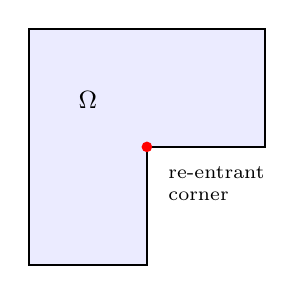
\begin{tikzpicture}[scale=1.5]
\fill[blue!8] (0,0) -- (1,0) -- (1,1) -- (-1,1) -- (-1,-1) -- (0,-1) -- cycle;
\draw[thick] (0,0) -- (1,0) -- (1,1) -- (-1,1) -- (-1,-1) -- (0,-1) -- cycle;
\fill[red] (0,0) circle (0.045);
\node[font=\scriptsize,anchor=west] at (0.1,-0.22) {re-entrant};
\node[font=\scriptsize,anchor=west] at (0.1,-0.42) {corner};
\node[font=\small] at (-0.5,0.4) {$\Omega$};
\end{tikzpicture}
\end{center}
\end{column}
\end{columns}
\end{frame}

\begin{frame}{What ``adaptive'' actually means}
\textbf{1. A local error indicator $\eta_K$.} A computable proxy for how much
error lives in element $K$. We use the gradient-jump indicator:
$$\eta_K^2 = \tfrac{1}{2}\sum_{e \in \partial K \cap \Omega^\circ}
   h_e \big| [\![ \nabla u_h \cdot n_e ]\!] \big|^2.$$
P1 gradients are discontinuous across edges, and the size of the jump
correlates with local error.

\vspace{0.8em}
\textbf{2. Dörfler marking.} Pick a bulk fraction $\theta \in (0,1)$. Mark the
smallest set $\mathcal{M}$ whose squared indicators capture a fraction $\theta$
of the total:
$$\sum_{K \in \mathcal{M}} \eta_K^2 \ \geq\ \theta \sum_K \eta_K^2.$$

\vspace{0.3em}
{\small Sort descending, walk the list until the running sum hits
$\theta \cdot \text{total}$, refine what you walked past. $\theta = 0.5$ is the
textbook default; smaller $\theta$ focuses on the worst offenders, larger
$\theta$ approaches uniform refinement.}
\end{frame}

\begin{frame}[fragile]{Tools the FEM agent gets}
Each takes a \code{mesh\_id} and returns a dict.

\vspace{0.5em}
\begin{itemize}\itemsep3pt
  \item \code{solve\_poisson(mesh\_id)} $\to$ \code{\{dofs, H1\_error\}}
  \item \code{local\_indicators(mesh\_id)} $\to$ summary stats of $\eta_K$
  \item \code{uniform\_refine(mesh\_id)} $\to$ new mesh id
  \item \code{refine\_by\_threshold(mesh\_id, theta)} $\to$ Dörfler-mark and refine
  \item \code{check\_convergence\_rate()} $\to$ log-log slope of the last 3 solves
  \item \code{stop(reason)}
\end{itemize}

\vspace{1em}
\textbf{Guardrails, in the tools:}
\begin{itemize}\itemsep2pt
  \item \code{MAX\_DOFS = 20000} --- a refinement that would exceed it returns an
        error observation instead of allocating.
  \item Every dispatch is \code{try/except} wrapped.
  \item \code{stop} is the only terminal tool.
\end{itemize}
\end{frame}

% ===========================================================================
\section{Reliability}

\begin{frame}[plain]
\begin{center}
\Huge\bfseries Reliability
\vspace{0.8em}

\large\mdseries or: agents are confidently wrong
\end{center}
\end{frame}

\begin{frame}{The failure mode that should actually worry you}
A crashed tool call is \emph{fine}. You see a traceback; the model retries.

\vspace{1em}
\begin{center}\large
The dangerous output is a \hl{plausible number with a confident summary}
and a bug upstream of both.
\end{center}

\vspace{1em}
In our setting, all of these produce clean-looking convergence plots:
\begin{itemize}\itemsep3pt
  \item the agent refines toward the wrong corner and the error still decreases;
  \item the error \emph{estimate} is fine but the solver has a sign error in the load;
  \item the reference energy is computed on too coarse a mesh, so every error looks small;
  \item the agent stops early and reports the tolerance as met.
\end{itemize}

\vspace{1em}
None of these announce themselves. \hl{Something independent has to check.}
\end{frame}

\begin{frame}{The verifier pattern}
\begin{center}
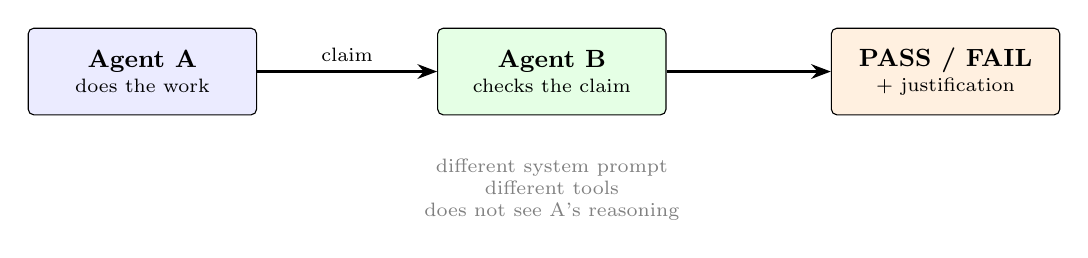
\begin{tikzpicture}[
  n/.style={draw,rounded corners=2pt,minimum width=2.9cm,minimum height=1.1cm,font=\small,align=center},
  ar/.style={-{Stealth[length=2.5mm]},thick}]
\node[n,fill=blue!8]   (a) at (0,0)   {\textbf{Agent A}\\[-2pt]\scriptsize does the work};
\node[n,fill=green!10] (v) at (5.2,0) {\textbf{Agent B}\\[-2pt]\scriptsize checks the claim};
\node[n,fill=orange!12](r) at (10.2,0){\textbf{PASS / FAIL}\\[-2pt]\scriptsize + justification};
\draw[ar] (a) -- node[above,font=\scriptsize]{claim} (v);
\draw[ar] (v) -- (r);
\node[font=\scriptsize,gray,align=center] at (5.2,-1.5)
  {different system prompt\\different tools\\does not see A's reasoning};
\end{tikzpicture}
\end{center}

\vspace{0.8em}
A verifier is just another agent. What makes it useful is what it is
\emph{denied}:

\begin{itemize}\itemsep3pt
  \item It does not see how the answer was produced --- only the claim.
  \item It has its \hl{own tools}, ideally sharing no code path with A's.
  \item Its system prompt rewards finding problems, not agreeing.
\end{itemize}

\vspace{0.5em}
{\small\color{gray}If A and B share the buggy solver, B will happily confirm the
bug. Independence is a property of the \emph{tools}, not the prompt.}
\end{frame}

\begin{frame}{Two verifiers we actually run}
\textbf{Verifier 1 --- manufactured solutions (for the FEM task).}

Pick a smooth $u_\text{exact}$, compute $f = -\Delta u_\text{exact}$
symbolically, solve with $u_h = u_\text{exact}$ on $\partial\Omega$, and measure
the error. For smooth $u_\text{exact}$ and P1 elements the rates are known:
$\|u-u_h\|_{L^2} = O(h^2)$, $|u-u_h|_{H^1} = O(h)$.

{\small The agent \emph{chooses} $u_\text{exact}$ --- which is itself a small
test of whether it understands the problem. A verifier that picks
$u = x + y$ has proven nothing, since P1 reproduces it exactly.}

\vspace{1em}
\textbf{Verifier 2 --- an oracle integrator (for the projectile task).}

The simulator uses \code{odeint} at default tolerance. The verifier re-integrates
the claimed optimum with \code{solve\_ivp(method="RK45", rtol=1e-10)} and reports
the discrepancy --- catching the case where the ``optimum'' is an artifact of
integration error rather than physics.

\vspace{1em}
\begin{center}
\hl{Both are ordinary numerical-methods practice.} The agent framing changes
nothing about what makes a result trustworthy.
\end{center}
\end{frame}

\begin{frame}{Where verification belongs}
Recall the LangGraph exemplar. This is why it was the exemplar.

\vspace{0.8em}
\begin{center}
\begin{tabular}{@{}ll@{}}
\toprule
\textbf{Verification as\ldots} & \textbf{What you get} \\
\midrule
a line in the system prompt & a suggestion, followed most of the time \\
a tool the agent may call & used when the agent feels uncertain \\
\hl{a node in a graph} & \hl{runs every time, or the result never ships} \\
\bottomrule
\end{tabular}
\end{center}

\vspace{1.2em}
The pattern and the reliability requirement are the same decision.
Choosing LangGraph over ReAct for the production FEM workflow \emph{is}
choosing to make verification non-optional.

\vspace{1em}
\begin{center}\small\color{gray}
This is the thread that connects the framework zoo to the engineering:
you don't pick a framework by taste, you pick it by which guarantee you need.
\end{center}
\end{frame}

% ===========================================================================
\section{Hands on}

\begin{frame}{Hands-on: what you'll build}
\textbf{Notebook \code{01\_agentic\_patterns.ipynb}} --- the zoo
\begin{itemize}\itemsep2pt\small
  \item \S1--\S5: each pattern, twice (framework syntax + ${\sim}15$ lines from scratch)
  \item \S6: \textbf{ReAct vs.\ MPC head-to-head} on the projectile, same budget
  \item \S7: \code{scipy.optimize} baseline --- the result that keeps us honest
\end{itemize}

\vspace{0.8em}
\textbf{Notebook \code{02\_agent\_hackathon.ipynb}} --- the FEM hackathon
\begin{itemize}\itemsep2pt\small
  \item \textbf{A1}: uniform-refinement agent (\code{uniform\_refine} only)
  \item \textbf{A2}: adaptive agent (Dörfler marking, $\theta = 0.5$)
  \item \textbf{A3}: rate-checking agent (adapts $\theta$ when the rate drops)
  \item \textbf{V}: manufactured-solution verifier
\end{itemize}

\vspace{0.8em}
\begin{center}
Every TODO has a worked solution one cell below. \hl{Use it.}
Reading a good system prompt is the fastest way to learn to write one.
\end{center}
\end{frame}

\begin{frame}{Stretch goals}
If you finish early, or want somewhere to go afterward:

\vspace{0.8em}
\begin{itemize}\itemsep5pt
  \item \textbf{Swap the backend.} Point the shim at Anthropic or OpenAI and see
        what changes in the tool-call round trip. (Answer: less than you'd expect.)
  \item \textbf{Break a tool on purpose.} Introduce a sign error in the load
        vector. Does your verifier catch it? Does the convergence plot?
  \item \textbf{Wire the FEM tools as a real graph.} Take the A2 agent and put
        the verifier on a conditional edge so a FAIL routes to further refinement.
  \item \textbf{Adversarial verifier.} Rewrite the verifier's system prompt to
        reward finding problems. Compare its pass rate against the neutral one.
  \item \textbf{Serve the FEM tools over MCP} and drive them from a client that
        isn't this notebook.
\end{itemize}
\end{frame}

% ===========================================================================
\begin{frame}{Taking it further}
\textbf{Agent patterns}
\begin{itemize}\itemsep1pt\small
  \item ReAct --- Yao et al.\ 2022, \url{https://arxiv.org/abs/2210.03629}
  \item LangGraph --- \url{https://langchain-ai.github.io/langgraph/}
  \item AutoGen --- \url{https://microsoft.github.io/autogen/}
  \item Model Context Protocol --- \url{https://modelcontextprotocol.io}
  \item smolagents (minimal framework) --- \url{https://huggingface.co/docs/smolagents}
\end{itemize}

\vspace{0.5em}
\textbf{Agents doing science}
\begin{itemize}\itemsep1pt\small
  \item FunSearch --- \emph{Nature} 625, 2024; AlphaEvolve --- DeepMind, 2025
  \item ChemCrow --- \url{https://arxiv.org/abs/2304.05376}
  \item Coscientist --- \emph{Nature} 624, 2023
  \item Sakana AI Scientist --- \url{https://sakana.ai/ai-scientist/}
\end{itemize}

\vspace{0.5em}
\textbf{Numerics}
\begin{itemize}\itemsep1pt\small
  \item scikit-fem --- \url{https://scikit-fem.readthedocs.io/}
  \item Dörfler, \emph{SIAM J. Numer. Anal.} 33(3), 1996
\end{itemize}
\end{frame}

\begin{frame}[plain]
\begin{center}
\vspace{2em}
{\Huge\bfseries Let's go.}

\vspace{1.5em}
{\large Open \code{01\_agentic\_patterns.ipynb} and run Part 0.}

\vspace{3em}
{\small\color{gray} Materials: \code{github.com/natrask/AESCAPE}}
\end{center}
\end{frame}

\end{document}
